\documentclass{article}
\usepackage[utf8]{inputenc}
\usepackage[english, ukrainian]{babel}
\usepackage{fontsize}
\usepackage{geometry}
\usepackage{amsthm}
\usepackage{amsfonts}
\usepackage{graphicx}
\usepackage[ruled]{algorithm2e}
\usepackage{hyperref}
\usepackage{biblatex}
\usepackage{csquotes}
\usepackage{mathtools}
\usepackage{amsmath}
\usepackage{amssymb}
\usepackage{bbm}
\usepackage{tabularx}
\usepackage{xcolor}

\usepackage{tikz}
\usetikzlibrary{decorations.pathmorphing}

\usepackage{enumitem}
\usepackage{nicefrac}

\usetikzlibrary{patterns}

\usepackage{diagbox}
\usepackage{longtable}

\usepackage{float}


\usepackage{enumitem}
\usepackage{nicefrac}

\usepackage{listings}
\definecolor{codegreen}{rgb}{0,0.6,0}
\definecolor{codegray}{rgb}{0.5,0.5,0.5}
\definecolor{codepurple}{rgb}{0.58,0,0.82}
\definecolor{backcolour}{rgb}{0.95,0.95,0.92}

\lstdefinestyle{mystyle}{
    backgroundcolor=\color{backcolour},   
    commentstyle=\color{codegreen},
    keywordstyle=\color{magenta},
    numberstyle=\tiny\color{codegray},
    stringstyle=\color{codepurple},
    basicstyle=\ttfamily\footnotesize,
    breakatwhitespace=false,         
    breaklines=true,                 
    captionpos=b,                    
    keepspaces=true,                 
    numbers=left,                    
    numbersep=5pt,                  
    showspaces=false,                
    showstringspaces=false,
    showtabs=false,                  
    tabsize=2
}

\lstset{style=mystyle}
\hypersetup{colorlinks=true, linkcolor=[RGB]{255, 3, 209}, citecolor={black}}

\graphicspath{ {../Images/} }

\begin{document}
    \begin{titlepage}
        \begin{center}
        $\newline$
        \vspace{3.3cm}
        
        {\LARGE\textbf{Лабораторна робота №3\\"Реалізація алгоритму оптимізації роєм часток для пошуку глобального мінімуму функції."}}
        \vspace{10cm}
        \begin{flushright}
            \textbf{Роботу виконав:}\\Климентьєв Максим \\3-го курсу\\групи ФІ-21
        \end{flushright}
        \end{center}
    \end{titlepage}
    \newpage

    \pagenumbering{gobble}
    \tableofcontents
    \cleardoublepage
    \pagenumbering{arabic}
    \setcounter{page}{3}

    \newpage

    \section{Опис набору даних. Візуалізація прикладів з набору даних.}
    \textbf{100} різних об'єктів, зображених з кутом обертання --- \textbf{від 0 до 360 з кроком 5}

    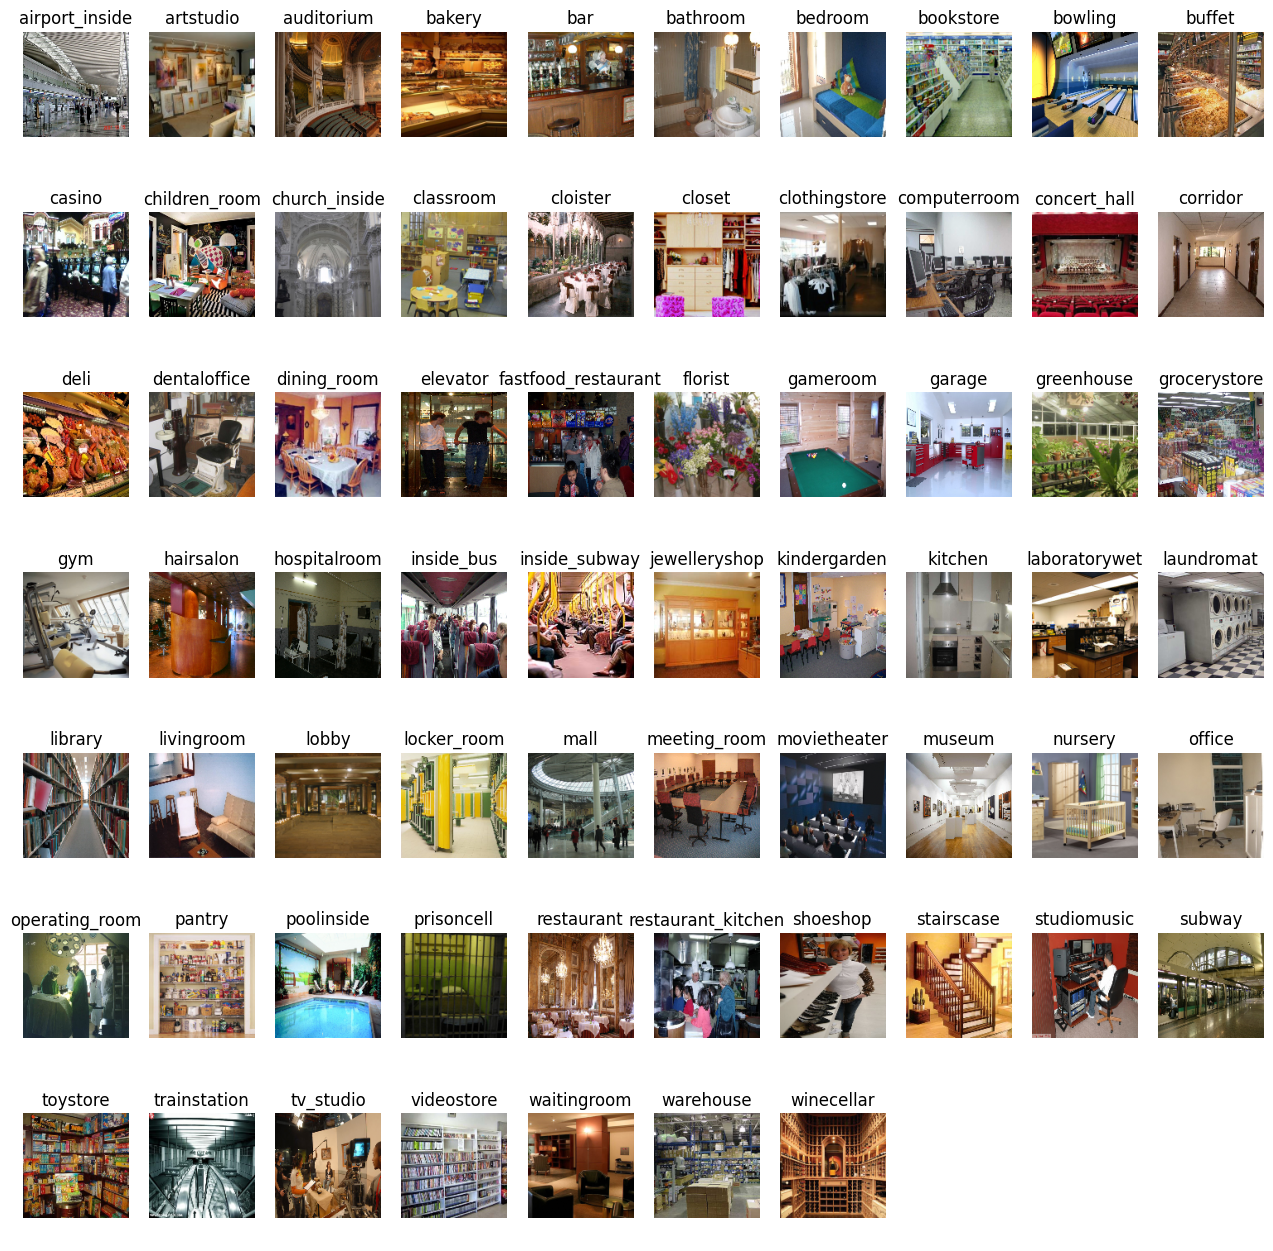
\includegraphics[width=\textwidth]{Types.png}
    \newpage

    \section{Опис базової архітектури.}
    \subsection{Архітектура нейронної мережі, кількість параметрів.}
    \begin{enumerate}
        \item 1 Conv2D 64:
            \begin{table}[h!]
                \begin{tabular}{| c | c | c |}
                    \hline
                    Layer (type) & Output Shape & Param \\
                    \hline
                    conv2d & (None, 64, 64, 64) & 1,792 \\
                    \hline
                    batch\_normalization & (None, 64, 64, 64) & 256 \\
                    \hline
                    max\_pooling2d & (None, 16, 16, 64) & 0 \\
                    \hline
                    flatten & (None, 16384) & 0 \\
                    \hline
                    dense & (None, 256) &  4,194,560 \\
                    \hline
                    dense & (None, 100) &  25,700 \\
                    \hline
                \end{tabular}
            \end{table}

            Total params: 4,222,308 (16.11 MB)

            Trainable params: 4,222,180 (16.11 MB)

            Non-trainable params: 128 (512.00 B)
        
            \item 1 Conv2D 64 + Dropout:
            \begin{table}[h!]
                \begin{tabular}{| c | c | c |}
                    \hline
                    Layer (type) & Output Shape & Param \\
                    \hline
                    conv2d & (None, 64, 64, 64) & 1,792 \\
                    \hline
                    batch\_normalization & (None, 64, 64, 64) & 256 \\
                    \hline
                    max\_pooling2d & (None, 16, 16, 64) & 0 \\
                    \hline
                    flatten & (None, 16384) & 0 \\
                    \hline
                    dense & (None, 256) &  4,194,560 \\
                    \hline
                    dropout & (None, 256) & 0 \\
                    \hline
                    dense & (None, 100) &  25,700 \\
                    \hline
                \end{tabular}
            \end{table}

            Total params: 4,222,308 (16.11 MB)

            Trainable params: 4,222,180 (16.11 MB)

            Non-trainable params: 128 (512.00 B)
        
        \newpage
            \item 1 Conv2D 32:
            \begin{table}[h!]
                \begin{tabular}{| c | c | c |}
                    \hline
                    Layer (type) & Output Shape & Param \\
                    \hline
                    conv2d & (None, 64, 64, 32) & 896 \\
                    \hline
                    batch\_normalization & (None, 64, 64, 32) & 128 \\
                    \hline
                    max\_pooling2d & (None, 16, 16, 32) & 0 \\
                    \hline
                    flatten & (None, 8192) & 0 \\
                    \hline
                    dense & (None, 256) & 2,097,408 \\
                    \hline
                    dense & (None, 100) &  25,700 \\
                    \hline
                \end{tabular}
            \end{table}

            Total params: 2,124,132 (8.10 MB)

            Trainable params: 2,124,068 (8.10 MB)

            Non-trainable params: 64 (256.00 B)
        
            \item 1 Conv2D 32 + Dropout:
            \begin{table}[h!]
                \begin{tabular}{| c | c | c |}
                    \hline
                    Layer (type) & Output Shape & Param \\
                    \hline
                    conv2d & (None, 64, 64, 32) & 896 \\
                    \hline
                    batch\_normalization & (None, 64, 64, 32) & 128 \\
                    \hline
                    max\_pooling2d & (None, 16, 16, 32) & 0 \\
                    \hline
                    flatten & (None, 8192) & 0 \\
                    \hline
                    dense & (None, 256) & 2,097,408 \\
                    \hline
                    dropout & (None, 256) & 0 \\
                    \hline
                    dense & (None, 100) &  25,700 \\
                    \hline
                \end{tabular}
            \end{table}

            Total params: 2,124,132 (8.10 MB)

            Trainable params: 2,124,068 (8.10 MB)

            Non-trainable params: 64 (256.00 B)
        
        \newpage
            \item 2 Conv2D:
            \begin{table}[h!]
                \begin{tabular}{| c | c | c |}
                    \hline
                    Layer (type) & Output Shape & Param \\
                    \hline
                    conv2d & (None, 64, 64, 64) & 1,792 \\
                    \hline
                    batch\_normalization & (None, 64, 64, 64) & 256 \\
                    \hline
                    max\_pooling2d & (None, 16, 16, 64) & 0 \\
                    \hline
                    conv2d & (None, 64, 64, 128) & 73,856 \\
                    \hline
                    batch\_normalization & (None, 64, 64, 128) & 512 \\
                    \hline
                    max\_pooling2d & (None, 16, 16, 128) & 0 \\
                    \hline
                    flatten & (None, 2048) & 0 \\
                    \hline
                    dense & (None, 256) & 524,544 \\
                    \hline
                    dense & (None, 100) &  25,700 \\
                    \hline
                \end{tabular}
            \end{table}

            Total params: 626,660 (2.39 MB)

            Trainable params: 626,276 (2.39 MB)
            
            Non-trainable params: 384 (1.50 KB)
        
            \item 2 Conv2D + Dropout:
            \begin{table}[h!]
                \begin{tabular}{| c | c | c |}
                    \hline
                    Layer (type) & Output Shape & Param \\
                    \hline
                    conv2d & (None, 64, 64, 64) & 1,792 \\
                    \hline
                    batch\_normalization & (None, 64, 64, 64) & 256 \\
                    \hline
                    max\_pooling2d & (None, 16, 16, 64) & 0 \\
                    \hline
                    conv2d & (None, 64, 64, 128) & 73,856 \\
                    \hline
                    batch\_normalization & (None, 64, 64, 128) & 512 \\
                    \hline
                    max\_pooling2d & (None, 16, 16, 128) & 0 \\
                    \hline
                    flatten & (None, 2048) & 0 \\
                    \hline
                    dense & (None, 256) & 524,544 \\
                    \hline
                    dropout & (None, 256) & 0 \\
                    \hline
                    dense & (None, 100) &  25,700 \\
                    \hline
                \end{tabular}
            \end{table}

            Total params: 626,660 (2.39 MB)

            Trainable params: 626,276 (2.39 MB)

            Non-trainable params: 384 (1.50 KB)
        
        \newpage

            \item Elu:
            \begin{table}[h!]
                \begin{tabular}{| c | c | c |}
                    \hline
                    Layer (type) & Output Shape & Param \\
                    \hline
                    conv2d & (None, 64, 64, 64) & 1,792 \\
                    \hline
                    batch\_normalization & (None, 64, 64, 64) & 256 \\
                    \hline
                    max\_pooling2d & (None, 16, 16, 64) & 0 \\
                    \hline
                    flatten & (None, 16384) & 0 \\
                    \hline
                    dense & (None, 256) &  4,194,560 \\
                    \hline
                    dense & (None, 100) &  25,700 \\
                    \hline
                \end{tabular}
            \end{table}

            Total params: 4,222,308 (16.11 MB)

            Trainable params: 4,222,180 (16.11 MB)

            Non-trainable params: 128 (512.00 B)
        
            \item Gelu:
            \begin{table}[h!]
                \begin{tabular}{| c | c | c |}
                    \hline
                    Layer (type) & Output Shape & Param \\
                    \hline
                    conv2d & (None, 64, 64, 64) & 1,792 \\
                    \hline
                    batch\_normalization & (None, 64, 64, 64) & 256 \\
                    \hline
                    max\_pooling2d & (None, 16, 16, 64) & 0 \\
                    \hline
                    flatten & (None, 16384) & 0 \\
                    \hline
                    dense & (None, 256) &  4,194,560 \\
                    \hline
                    dense & (None, 100) &  25,700 \\
                    \hline
                \end{tabular}
            \end{table}

            Total params: 4,222,308 (16.11 MB)

            Trainable params: 4,222,180 (16.11 MB)

            Non-trainable params: 128 (512.00 B)
        
            \item Gelu + Learning Rate:
            \begin{table}[h!]
                \begin{tabular}{| c | c | c |}
                    \hline
                    Layer (type) & Output Shape & Param \\
                    \hline
                    conv2d & (None, 64, 64, 64) & 1,792 \\
                    \hline
                    batch\_normalization & (None, 64, 64, 64) & 256 \\
                    \hline
                    max\_pooling2d & (None, 16, 16, 64) & 0 \\
                    \hline
                    flatten & (None, 16384) & 0 \\
                    \hline
                    dense & (None, 256) &  4,194,560 \\
                    \hline
                    dense & (None, 100) &  25,700 \\
                    \hline
                \end{tabular}
            \end{table}

            Total params: 4,222,308 (16.11 MB)

            Trainable params: 4,222,180 (16.11 MB)

            Non-trainable params: 128 (512.00 B)
\end{enumerate}

\newpage
    \subsection{Точність класифікації.}

    \foreach \x in {1,2,...,9}
    {
        \begin{figure}[H]
            \centering
            \includegraphics[width=0.5\linewidth]{accuracy_\x.png}
            \caption{\x}
        \end{figure}
    }

    \newpage
    \subsection{Візуалізація функцій втрат (тестовий та тренінговий набір).}

    \foreach \x in {1,2,...,9}
    {
        \begin{figure}[H]
            \centering
            \includegraphics[width=0.5\linewidth]{loss_\x.png}
            \caption{\x}
        \end{figure}
    }
    \newpage

    % \subsection{Параметри точності класифікації.}

    \section{Опис експериментів.}
    \subsection{Які зміни було внесено.}
    \begin{itemize}
        \item Базова версія - 1 Conv2D 64
        \item Run №2 - 1 Conv2D 64 + Dropout

        \item Run №3 - 1 Conv2D 32
        \item Run №4 - 1 Conv2D 32 + Dropout

        \item Run №5 - 2 Conv2D
        \item Run №6 - 2 Conv2D + Dropout

        \item Run №7 - Elu
        \item Run №8 - Gelu

        \item Run №9 - Gelu + Learning Rate
    \end{itemize}

    \subsection{Висновки: як це вплинуло на результат, процес тренування, ...}
        Більше Conv2D потребує більше епох для того щоб отримати таку ж точність як для одного Conv2D

    \section{Результати порівняння.}
    \begin{table}[h!]
        \begin{tabular}{| c | c | c | c | c | c | c | c |}
            \hline
            Опис & Dropout & More Conv2D & Accuracy & Loss & Training Time & Top2 & Activation Func \\
            \hline
            Базова & - & - & 99 & 13 & 19 & 1 & Relu \\
            \hline
            Run №2 & + & - & 99 & 9 & 29 & 1 & Relu \\
            \hline
            Run №3 & - & - & 99 & 11 & 9 & 1 & Relu \\
            \hline
            Run №4 & + & - & 0 & 0 & 0 & 0 & Relu \\
            \hline
            Run №5 & - & + & 0 & 0 & 0 & 0 & Relu \\
            \hline
            Run №6 & + & + & 0 & 0 & 0 & 0 & Relu \\
            \hline
            Run №7 & - & - & 0 & 0 & 0 & 0 & Elu \\
            \hline
            Run №8 & - & - & 0 & 0 & 0 & 0 & Gelu \\
            \hline
            Run №9 & - & - & 0 & 0 & 0 & 0 & Gelu \\
            \hline
        \end{tabular}
    \end{table}

    \section{Висновки.}
    Базва версія є найкращою

\end{document}